\label{sec:DiIDiDEphB1}
Previous work from our lab detailed the decussation and targeting phenotypes in the EphB1\textsuperscript{-/-} mutant, leaving the optic tract largely unexamined.
I therefore conducted whole eye anterograde labeling of the retinal projections the in EphB1\textsuperscript{-/-} retinogeniculate pathway in the same way as done in Chapter 2 to assess ipsi/contra RGC axon organization in the wild-type (see Section~\ref{sec:DiIDiDWT}).
Figure~\ref{EphB1WTDiIDiD} shows the eye-specific axon order in the EphB1\textsuperscript{-/-} optic tract compared to equivalent sections from the wild-type tract at P0.
In both frontal (Figure~\ref{EphB1WTDiIDiD}B) and horizontal (Figure~\ref{EphB1WTDiIDiD}C) planes, it is clear that the remaining ipsi RGC axons are positioned in the lateral aspect of the optic tract, similar to ipsi axons in the wild-type tract.

However, ipsi axons in the EphB1\textsuperscript{-/-} optic tract appear less well fasciculated than in the wild-type tract, with more gaps apparent between axons and occupying a more diffusely spread area in the lateral tract.
Additionally, ipsi RGC axons appear less well organized overall, with a few axons straying more medially, away from the main area of ipsi axons.
This is most clearly evident in the horizontal plane, shown in Figure~\ref{EphB1WTDiIDiD}C.
\begin{figure}[hbtp]
    \begin{center}
        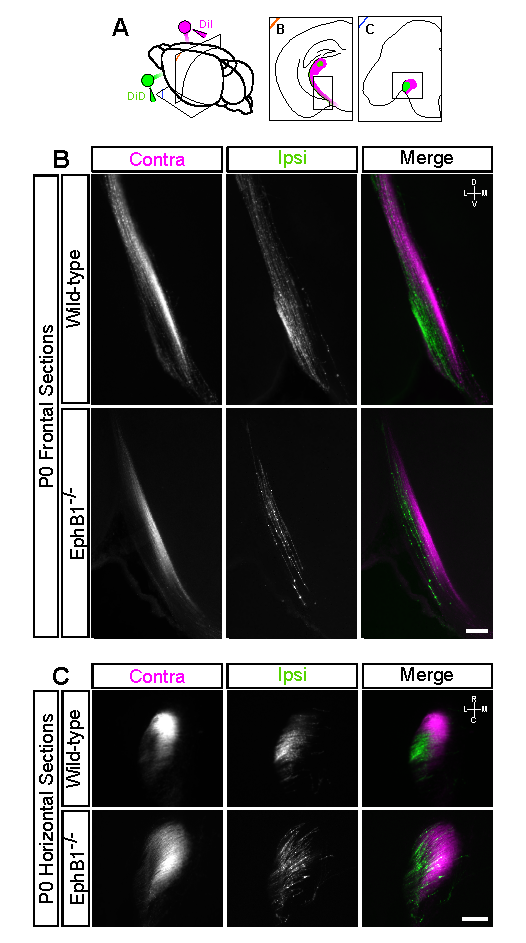
\includegraphics{Figures/EphB1_WT_DiIDiDv1.pdf}
        \caption[Remaining ipsi RGC axons in the EphB1\textsuperscript{-/-} optic tract are poorly fasciculated.]
        {Remaining ipsi RGC axons in the EphB1\textsuperscript{-/-} optic tract are poorly fasciculated.
        A) Labeling schema: DiI and DiD crystals were applied to the optic nerve head of right and left eyes, respectively, in fixed P0 heads.
        Samples were sectioned 75$\mu$m thick in frontal (B) or horizontal (C) planes for imaging and analysis.
        In both planes, ipsi RGC axons (green) in the EphB1\textsuperscript{-/-} tract are fewer in number and appear poorly fasciculated compared to wild-type (WT) ipsi axons.
        In the horizontal plane (C), EphB1\textsuperscript{-/-} ipsi axons appear less well organized than WT ipsi axons, often straying outside of the lateral zone of the tract.
        D=dorsal, V=ventral, R=rostral, C=caudal, M=medial, L=lateral.
        Scale=100$\mu$m.
        }
        \label{EphB1WTDiIDiD}
    \end{center}
\end{figure}

Thus, loss of EphB1 does not affect the positioning of ipsi RGC axons to the lateral edge of the optic tract.
EphB1 may, however, be involved in the fasciculation of the ipsi cohort and/or the segregation of ipsi and contra RGC axon cohorts.
%(Section~\ref{sec:EphB1invitro} directly tests fasciculation in EphB1\textsuperscript{-/-} retinal explants.)
Alternatively, what presents as defasciculation of ipsi axons in the EphB1\textsuperscript{-/-} optic tract may instead be a reflection of the reduction in number of ipsi axons.
A portion of the ipsi RGC cohort improperly crossed the chiasm and project into the contra tract in the EphB1\textsuperscript{-/-} mutant.
Thus, these genetically ipsi axons (i.e., Zic2\textsuperscript{+}) that behave as contra axons (due to loss of EphB1) may still bundle with the remaining ipsi axons - however, this cohort of aberrantly crossed axons cannot be visibly dissociated from the normal contra cohort in the current labeling scheme.
Thus, it is unclear if the appearance of reduced fasciculation in the remaining ipsi RGC axons is due to true defasciculation of this axonal cohort.
The next two sections present in vivo and in vitro evidence to address this issue.
